% 图 4.5 相邻格点磁矩 m_i, m_j 与夹角 phi_ij 的矢量几何
\documentclass[tikz,border=5pt]{standalone}
\usetikzlibrary{arrows.meta}
\usepackage{amsmath}
\usepackage{bm}
\usepackage{fontspec}
\setmainfont{Times New Roman}
\begin{document}
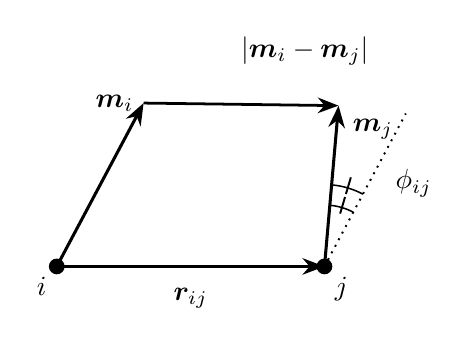
\begin{tikzpicture}[line width=0.8pt,>=Stealth]
% sites
\fill (0,0) circle (0.10);
\fill (3.4,0) circle (0.10);
\node[below left] at (0,0) {$i$};
\node[below right] at (3.4,0) {$j$};
% r_ij
\draw[line width=1.1pt,->] (0,0) -- (3.4,0);
\node[below] at (1.7,-0.14) {$\bm{r}_{ij}$};
% moments
\draw[line width=1.1pt,->] (0,0) -- (62:2.35);
\node[left] at (62:2.35) {$\bm{m}_i$};
\draw[line width=1.1pt,->] (3.4,0) -- ({3.4+2.05*cos(85)},{2.05*sin(85)});
\node[right] at ({3.4+2.05*cos(85)+0.05},{2.05*sin(85)-0.30}) {$\bm{m}_j$};
% dotted line through j parallel to m_i
\draw[dotted,line width=0.7pt] (3.4,0) -- ({3.4+2.20*cos(62)},{2.20*sin(62)});
% angle arcs with tick marks
\draw[line width=0.55pt] ([shift={(3.4,0)}]62:0.78) arc[start angle=62,end angle=85,radius=0.78];
\draw[line width=0.55pt] ([shift={(3.4,0)}]62:1.04) arc[start angle=62,end angle=85,radius=1.04];
\draw[line width=0.7pt] ([shift={(3.4,0)}]73.5:0.70) -- ([shift={(3.4,0)}]73.5:0.92);
\draw[line width=0.7pt] ([shift={(3.4,0)}]73.5:0.96) -- ([shift={(3.4,0)}]73.5:1.18);
\node at ([shift={(3.4,0)}]43:1.55) {$\phi_{ij}$};
% vector difference triangle
\coordinate (mi) at (62:2.35);
\coordinate (mj) at ({3.4+2.05*cos(85)},{2.05*sin(85)});
\draw[line width=1.0pt,->] (mi) -- (mj);
\node[above] at (3.15,2.42) {$|\bm{m}_i-\bm{m}_j|$};
\end{tikzpicture}
\end{document}
